\documentclass[paper=a4, fontsize=12pt, xcolor=dvipsnames]{scrartcl} % A4 paper and 11pt font size

\usepackage[utf8]{inputenc}
\usepackage{cmbright}
\usepackage[english]{babel} 
\usepackage{amsmath}
\usepackage{braket}
\usepackage{float} %placing floats(H)
\usepackage{graphicx}
\usepackage[top=2in, bottom=1.5in, left=1.25in, right=1in]{geometry} %setting merges
\usepackage{fancyhdr}%headers/footers
\pagestyle{fancy} 
\usepackage[font={color=gray1},figurename=Fig.,labelfont={color=blue}]{caption}
\usepackage{hyperref}
\usepackage{xfrac}


% BIBLIOGRAPHY
% using biblatex and biber
\usepackage[
style=nature,              % Zitierstil
isbn=false,                % ISBN nicht anzeigen, gleiches geht mit nahezu allen anderen Feldern
pagetracker=true,          % ebd. bei wiederholten Angaben (false=ausgeschaltet, page=Seite, spread=Doppelseite, true=automatisch)
maxbibnames=50,            % maximale Namen, die im Literaturverzeichnis angezeigt werden (ich wollte alle)
maxcitenames=3,            % maximale Namen, die im Text angezeigt werden, ab 4 wird u.a. nach den ersten Autor angezeigt
autocite=inline,           % regelt Aussehen für \autocite (inline=\parancite)
block=space,               % kleiner horizontaler Platz zwischen den Feldern
backref=false,              % Seiten anzeigen, auf denen die Referenz vorkommt
backrefstyle=three+,       % fasst Seiten zusammen, z.B. S. 2f, 6ff, 7-10
date=short,                % Datumsformat
hyperref=true,
backend = biber
]{biblatex}
\setlength{\bibitemsep}{1em}     % Abstand zwischen den Literaturangaben
\setlength{\bibhang}{2em}        % Einzug nach jeweils erster Zeile
\bibliography{bibliography}

\begin{document}
  \section{Introduction}
The Nobel prize in physics 2012 was awarded jointly to the French physicist
Serge Haroche and the American physicist David Wineland.
According to the Nobel jury they received it ``for ground-breaking experimental
methods that enable measuring and manipulation of individual quantum systems''.
Serge Haroche spent most of his life researching at the École Normale Supérieure
in Paris. There he created photon traps, i.e. cavities, in which microwave
photons could be stored up to half a second~\cite{haroche2007QuantumJumps}. To
probe the wave function of the photons, he sent in groups of or single atoms to
see how they would interact with the light. In this way he unveiled many of the
interesting effects of the quantum nature of light. David Wineland spent most of
his scientific life on the other side of the Atlantic, at the National Institute
of Standards and Technology in Boulder, Colorado. His drive was to invent better
methods to slow down and
isolate ions as this allowed frequency measurements of
higher and higher precision. To achieve this, he used sophisticated setups
combining ion traps with high precision lasers. 

But if one of the laureates dedicated his research to photons and the other one
to ions, why did they share the Nobel prize? The answer to this question lies in
the congruence of their methods with respect to quantum mechanics. Haroche was
probing photons with atoms, Wineland examined the energy levels of atoms using
photons, but both were dealing with the same underlying effects of quantum
mechanics. This can be easily seen when one leaves aside their specific physical
objects of study (i.e. photons and ions) and inspects which abstract topics
they were dealing with. Both of them published papers about ``Schrödinger Cat
States''~\cite{brune1992manipulation, monroe1996schrodinger}, bringing to
physical experiment one of the most fundamental thought experiments of early
quantum mechanics. Both conducted experiments on many particle entanglement
~\cite{rauschenbeutel2000step, sackett2000experimental}. Both found ways to
engineer explicitly  non-classical states in their systems~\cite{meekhof1996generation,
deleglise2008reconstruction}. This list could be continued, but the message is
clear: each of them in their own fields found ways to answer fundamental issues
of quantum mechanics experimentally and on their way introduced countless new
methods to the physics community.

The outline of this term paper is as follows: first we will theoretically derive
the phenomenon of Rabi oscillations from the Jaynes-Cummings Hamiltonian, because
both, Haroche and Wineland, used it as a central method in their later
experiments (Sec.~\ref{sec:Theory}) . Then we will have a look at  each of the
laureate's early life and inspect some of their central experiments in order to
get an impression of their experimental creativity and innovation
(Sec.~\ref{sec:Haroche}~and~\ref{sec:Wineland}). A short conclusion will then be
given in Sec.~\ref{sec:Conclusion}.

  \section{Theory}
Some theoretical concepts of quantum optics are necessary to understand the ways
in which Serge Haroche and David Wineland experimentaly observed fundamental
quantum mechanical effects. This section aims to introduce the basic model of a
fully quantum mechanical description of atom-light interaction, the Jaynes-Cummings model, and
one of the most used results of it, namely Rabi oscillations.

\subsection{Jaynes-Cummings Hamiltonian}
Rabi cycles are a phenomenon that occurs when an atom interacts with light.
Both, Serge Haroche and David Wineland, investigated and made use of the
shifts in energylevels and relative phases of states that appear when a laser
shines in on an atom.  In
order give a useful and complete description of Raby cycles, one has to take into
account that the energy levels of the atom and of the photon field are
quantized. The first ``fully quantized'' approach for the case of coherent light
in a cavity and a two level system was given by Edwin Jaynes and Fred Cummings
in 1963 \cite{jaynes1963comparison}. To describe the system (following
\cite{gerry2005introductory}) 
we introduce the total Hamiltonian, consisting of the Hamiltonian for the 
 quantized photon field for a single mode, the Hamiltonian of the two level
 system consisting of a ground state $\ket{g}$ and an excited state $\ket{e}$ and the
 interaction Hamiltonian
\begin{align}
  \label{eq:JCM_H_tot}
  {\hat {H}}={\hat {H}}_{{{\text{field}}}}+{\hat {H}}_{{{\text{atom}}}}+{\hat
  {H}}_{{{\text{int}}}},
\end{align}
where, neglecting the zero point energies of field and atom,
\begin{align}
  \label{eq:JCM_H_field}
  \hat{H}_{\text{field}} &= \hbar \omega_{\text{f}}\, \hat{a}^\dagger
   \hat{a}\\
  \label{eq:JCM_H_atom}
  \hat{H}_{\text{atom}} &= \frac{\hbar \omega_a}{2} \, \hat{\sigma_3} \\
  \label{eq:JCM_H_int}
  \hat{H}_{\text{int}} &= \hbar \omega_{\text{int}} \left( \hat{\sigma}_+ +
\hat{\sigma}_-\right)\left(\hat{a} + \hat{a}^\dagger\right).
\end{align}
Here $\hat{a}^\dagger$ and $\hat{a}$ are the creation and annihilation operators
that appear in the quantization of the electromagnetic field\footnote{To solve
the free field equation of the elmg. field one usually uses the Fourier ansatz
$$A^\mu(x) = \int \text{d}\tilde{k} \sum_{\lambda=0}^3 \left[ a_\lambda(\vec{k})
\epsilon^\mu_\lambda(k)\text{e}^{-ikx} +
a^\dagger_\lambda(\vec{k})\epsilon^\mu_\lambda(k)^* \text{e}^{+ikx}\right], $$
where $\lambda$ goes over all possible polarizations. When demanding that
$A^\mu$ and its conjugate field $\pi^\nu$ obey the canonical quantization
relation, the resulting commutator relations for $a_\lambda$ and
$a_\lambda^\dagger$ allow the interpretation as creation and annihilation
operators.}, the Pauli matrix $\hat{\sigma_3} = \ket{e}\bra{e} - \ket{g}\bra{g}$
acts as the inversion operator of the atom, and the associated Pauli
matrices $\hat{\sigma}_+ = \ket{e}\bra{g}$ and $\hat{\sigma}_- = \ket{g}\bra{e}$
project any state $\ket{g}$ ($\ket{e}$) to $\ket{e}$ ($\ket{g}$) respectively
and can thus be seen as atomic transition operators. It is now useful to look at
the time evolution of the terms in the total Hamiltonian \eqref{eq:JCM_H_tot}.
To do so we switch to the interaction picture, using the Hamiltonian without
interaction $\hat{H}_0 = \hat{H}_{\text{atom}} + \hat{H}_{\text{field}}$ to
describe the time evolution of the operators. For the  annihilation operator we
have 
\begin{align}
  \label{eq:a_time_ev}
  \hat{a}(t) &= e^{i\hat{H_0}t/\hbar}\, \hat{a}(0)\, e^{-i\hat{H_0}t/\hbar}
  \nonumber \\
  \intertext{using the Baker-Campbell-Hausdorff formula, we obtain}
  &= \hat{a}(0) + \frac{it}{\hbar}\left[\hat{H}_0, \hat{a}\right] +
  \frac{1}{2!}\left(\frac{it}{\hbar}\right)^2\left[\hat{H}_0, \left[\hat{H}_0,
  \hat{a}\right] \right] + \dots \nonumber
  \intertext{The first commutator is $\left[\hat{H}_0, \hat{a}\right] = -\hbar \omega_f
  \hat{a}$ as $\hat{a}$ commutes with $\hat{H}_{\text{atom}}$ and
  $\left[\hat{a}^\dagger, \hat{a}\right]=-1$. The nested commutators will thus only add higher orders of $\omega_f$. The
time evolution then becomes}
&= \hat{a}(0) \left(1 - it\omega_f + (it\omega_f)^2 + \dots  \right) \nonumber
\\
&= \hat{a}(0) e^{-i\omega_f t}.\,\footnotemark
\end{align}
\footnotetext{By looking at the preceeding footnote
and considering that $kx$ is a scalar product of four-vectors but the
integration over $\text{d}\tilde{k}$ is only over the three spatial components,
we see that the time evolution behaviour is already built-in in this ansatz.}Correspondingly we obtain for the other operators
\begin{align}
  \label{eq:ops_time_ev}
  \hat{a}^\dagger(t) &= \hat{a}^\dagger(0)e^{i\omega_ft}\\
  \hat{\sigma}_\pm(t) &= \hat{\sigma}_\pm(0)e^{\pm i\omega_a t}
\end{align}
and therefore the full interaction Hamiltonian becomes
\begin{align}
  \label{eq:H_int_time_ev}
  \hat{H}_{\text{int}}(t) = \hbar \omega_{\text{int}} \left( \hat{\sigma}_+ \hat{a}
  \, e^{i(\omega_a-\omega_f)t} \right& + \hat{\sigma}_+ \hat{a}^\dagger\,
    e^{i(\omega_a+\omega_f)t}\nonumber\\ & \left\quad + \hat{\sigma}_-\hat{a}\, e^{-i(\omega_a+\omega_f)t}
+ \hat{\sigma}_-\hat{a}^\dagger \, e^{-i(\omega_a-\omega_f)t}\right).
\end{align}
Assuming that the photon frequency $\omega_f$ is close to the transition
frequency of the atom $\omega_a$, i.e. $\left| \omega_a-\omega_f \right|
\ll \omega_a+\omega_f $, the rotating wave approximation can be applied. This
means that all terms in $\hat{H}_{\text{int}}$ that oscillate with
$\omega_a+\omega_f$ are
neglected. Doing this and transforming back to the Schrödinger picture leaves us
with the total Hamiltonian
\begin{align}
  \label{eq:H_tot_rot_wave}
  \hat{H}_{\text{tot}}= \hbar \omega_f \hat{a}^\dagger \hat{a} + \frac{\hbar\omega_a}{2}\hat{\sigma}_3
  + \hbar \omega_{\text{int}}\left( \hat{\sigma}_+\hat{a} +
  \hat{\sigma}_-\hat{a}^\dagger  \right).
\end{align}
The last two terms can be seen as processes in which the atom aborbs or emmits
one photon from the field while respectively changing its internal energy state.

\subsection{Rabi Oscillations}
Having found a Hamiltonian that describes the interaction of an atom with light,
it is now interesting to investigate how this interaction influences the
dynamics of the system. The original states of atom and fiel will no longer be
eigenstates of the system and thus undergo a continuous oscillation, called Rabi
oscillation. Bot, Serge Haroche and David Wineland have made experimental use of
this effect in order to prepare and manipulate states. To describe the dynamics
it is first useful to split the Hamiltonian in \eqref{eq:H_tot_rot_wave} into
two parts, namely
\begin{align}
  \label{eq:H_I_H_II}
  \hat{H}_I &= \hbar\omega_f\underbrace{\left( \hat{a}^\dagger\hat{a} +
  \ket{e}\bra{e}\right)}_{\text{excitation number }\hat{N}_e} + \hbar \left( \frac{\omega_a}{2} -
\omega_f)\right)\underbrace{\left(\ket{e}\bra{e} +
\ket{g}\bra{g}\right)}_{\text{e$^-$ number projector }\hat{P}_e} \\
\hat{H}_{II} &= -\hbar \underbrace{\left(\omega_a -
\omega_f\right)\ket{g}\bra{g}}_{\equiv\Delta} +
\hbar\omega_{\text{int}}\left( \hat{\sigma}_+\hat{a} +
  \hat{\sigma}_-\hat{a}^\dagger  \right).
\end{align}
The first part $\hat{H}_I$ commutes with $\hat{H}_{\text{tot}}$ thus it is
conserved over time and any interesting dynamics of the system are described by
the second part. Let us now consider a state
\begin{align}
  \label{eq:psi_t}
  \ket{\psi(t)} = C_1(t)\ket{e}\ket{n} + C_2(t)\ket{g}\ket{n+1} 
\end{align}
with initial conditions $C_1(0) = 1$ and $C_2(0)=0$. The time evolution is
described by the time dependend Schrödinger equation
$i\hbar\frac{\text{d}}{\text{d}t}\ket{\psi(t)}
= \hat{H}_{II}\ket{\psi(t)}$. In the resonant case ($\Delta=0$) this can be
exactly solved and yields
\begin{align}
  \label{eq:psi_t_solution}
  C_1(t) &= \cos\left(\omega_{\text{int}}\sqrt{n+1}\,t\right) \\
  C_2(t) &= -i\sin\left(\omega_\text{int} \sqrt{n+1} \,t\right)
\end{align}

We see that the state of a two level system can be manipulated by sending in coherent
  light, a technique that is crucial for many quantum optics experiments. In this 
context a nomenclatur for pulses is established, describing to what extent the
light interacts with the atom. A pulse of light is called ``$ r\pi$-pulse'' ($r\in \mathbb{R}$)
if it interacts with an atom such that
\begin{align}
  \label{eq:r_pulse}
  \omega_{\text{int}}\sqrt{n+1}\, t = \frac{r \pi}{2}.
\end{align}
A commonly used type of pulse is for example the $\pi/2$-pulse that takes e.g. a
pure state $\ket{e}\ket{n}$ to a superposition
state $\frac{1}{\sqrt{2}}\left(\ket{e}\ket{n}-i\ket{g}\ket{n+1}\right)$. In the basis spanned by $\left\lbrace
\ket{e}\ket{n}, \ket{g}\ket{n+1}\right\rbrace$ a $\pi/2$-pulse can be
represented in matrix form as
\begin{align}
  \label{eq:pi_half_matrix}
U(\pi/2) = \frac{1}{\sqrt{2}}  
\begin{pmatrix*}[r] 
      1 & -i \\
      -i & 1
    \end{pmatrix*}.
\end{align}
The repeated action of a $\pi/2$-pulse on a two level system is shown
graphically in Fig.~\ref{fig:rabi_cycle_rep}. It should be noted that starting
from $\ket{e}\ket{n}$ and performing a full rabi cycle will introduce a global
phase of $-1$ to the system. However this phase is not of physical importance
when the two level system is closed and only measurable in comparison to a
reference system.\footnote{$\braket{e|\hat{O}|e} = \braket{e|(-1)\hat{O}(-1)|e}$
for any observable $\hat{O}$.}
\begin{figure}[h]
  \centering
  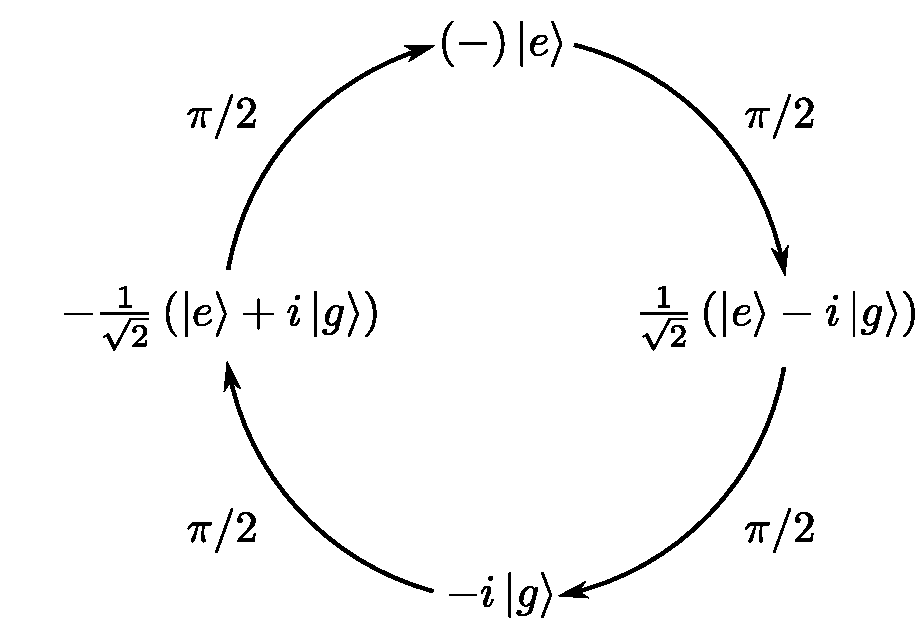
\includegraphics[width=.5\linewidth]{rabi_cycle_rep.pdf}
  \caption{Graphic representation of the action of a $\pi/2$-pulse on the state
    of a two level system. The photon number states (e.g. as in $\ket{e}\ket{n}$)
    are not shown explicitly. The $(-)$ in front of the excited state indicates
  the change of the total phase after one full cycle, which is of importance
only if there is another state to which it should be compared in measurement.}
  \label{fig:rabi_cycle_rep}
\end{figure}

\subsection{Dressed States}
\label{sec:DressedStates}
When we want to describe the dynamics of a two level system also in the
off-resonant case requires diagonalization of the Hamiltonian
\eqref{eq:H_tot_rot_wave}. The resulting eigenstates are called ``dressed
states'', a wording that suggests that they are atom states ``dressed in light'' in contrast
to the ``bare'' states of the atom without a light field. Using again the basis
$\left\lbrace \ket{e}\ket{n}, \ket{g}\ket{n+1}\right\rbrace$ we can represent
\eqref{eq:H_tot_rot_wave} as
\begin{align}
  \label{eq:H_tot_matrix}
  \hat{H}_{\text{tot}} = 
  \renewcommand*{\arraystretch}{2}
  \begin{pmatrix*}[c]
    n\omega_f + \frac{1}{2} \hbar\omega_a & \hbar\omega_{\text{int}} \sqrt{n+1}\\
    \hbar\omega_{\text{int}} \sqrt{n+1}\quad & (n+1)\omega_f - \frac{1}{2}\omega_a
  \end{pmatrix*}
\end{align}
and diagonalize it. From this we obtain the eigenenergies 
\begin{align}
  \label{eq:eigenergies}
  E_\pm = \hbar\omega_f\left(n+\frac{1}{2}\right) \pm \hbar\Omega_n(\Delta)
\end{align}
with the off resonant Rabi frequency
\begin{align}
  \label{eq:Omega_n}
  \Omega_n(\Delta) = \sqrt{\Delta^2 + 4 \omega_{\text{int}}^2(n+1)}.
\end{align}
The eigenenergies of the new eigenstates depend on the detuning of the light
with respect to the atom transition. This shift in the energy levels is often
referred to as the ``AC-Stark-shift''.
The corresponding eigenstates in the given basis are
\begin{align}
  \label{eq:eigenstates}
  \ket{n,+} &=  \cos(\Phi_n/2)\ket{e}\ket{n} +  \sin(\Phi_n/2) \ket{g}\ket{n+1}\\ 
  \ket{n,-} &=  -\sin(\Phi_n/2)\ket{e}\ket{n} +  \cos(\Phi_n/2) \ket{g}\ket{n+1} 
\end{align}
where the angle $\Phi_n$ is given by
\begin{align}
  \label{eq:phi_n}
  \Phi_n = \tan^{-1}\left( \frac{2\omega_{\text{int}}\sqrt{n+1}}{\Delta} \right)
\end{align}
which converges towards $\pi/2$ for $\Delta\rightarrow 0$. The dressed states
are now useful for many applications in the field of quantum optics. Given a
prepared state of a two level atom, one can determine the interaction of the
atom with (not necessarily resonant) incident light by expressing the initial
state in terms of the dressed states. As the dressed states are eigenstates of
the total Hamiltonian their time evolution is trivial under application of the
time evolution operator. In this way the dynamics can be calculated in the
dressed states basis and afterwards (if needed) transformed back to the initial
basis.

\subsection{Far Off Resonance Case}
The full Jaynes-Cummings Hamiltonian \eqref{eq:JCM_H_tot} without the rotating
wave approximation can also be treated for the far-off resonant case
$\Delta\gg\omega_a$. Interaction is in this case ruled by the effective
Hamiltonian 
\begin{align}
  \label{eq:H_eff}
  \hat{H}_{\text{eff}} = \hbar \chi \left[\hat{\sigma}_+\hat{\sigma_-} +
  \hat{a}^\dagger \hat{a}\sigma_3 \right],
\end{align}
where $\chi$ depends on the photon number $n$ and the detuning $\Delta$
\cite{gerry2005introductory}. Under this Hamiltonian a state
\begin{align}
  \label{eq:psi_evol_0}
  \ket{\Psi(0)} = \frac{1}{\sqrt{2}} \left(\ket{e}\ket{n} +
  \ket{g}\ket{n}\right)
\end{align}
will evolve according to 
\begin{align}
  \label{eq:psi_evol_t}
  \ket{\Psi(t)} = \frac{1}{\sqrt{2}} \left( \ket{e}\ket{n} + e^{-i\,\chi
  (\Delta,n)t} \ket{g}\ket{n}\right),
\end{align}
a time evolution that Serge Haroche used to non-destructively detect single
photons (see Sec.~\ref{sec:QND}).

  \section{Serge Haroche}


\begin{frame}[t]{Serge Haroche: Early life}
  \portraitpic{haroche.jpg}
  \visible<3>{
    \textpos{\linewidth}{0cm}{3cm}{\begin{quote}``I was a very good student,
    immediately at the head of my class in the Lycée Carnot''\end{quote}}
  }
  \visible<6>{\picpos{6cm}{1cm}{2.8cm}{lab_kastler_brossel.jpg}}
  \visible<7>{
    \textpos{\linewidth}{0cm}{3cm}{\begin{quote}``Enthralled by the mysterious beauty of the quantum
          world, it did not take me long to decide that I wanted to become a
        quantum physicist''\end{quote}}
  }

  \begin{minipage}[t][4cm][t]{\textwidth}
    \begin{itemize}
      \item<1-> Born in Casablanca, Morocco
      \item<2-> Parents move to Paris
      \item<4-> École préparatoires at Paris
      \item<5-> Accepted for École normale supérieure (ENS)
    \end{itemize}  
  \end{minipage}
  \begin{minipage}[t][0.2\textheight][t]{\textwidth}
    \begin{chronology}[10]{1940}{2016}{\textwidth}{5cm}
      \visible<1>{\event{1944}{24.02.1944}}
      \visible<2>{\event{1956}{'56}}                  
      \visible<4>{\event{1962}{'62}}                  
      \visible<5,7>{\event[1963]{1967}{'63 -- '67}}
      \visible<>{ \event[1967]{1972}{'67 -- '72}} 
      \visible<>{\event[1972]{1973}{'72 -- '73}}
      \visible<>{\event[1973]{1975}{'73 -- '75}}
      \visible<>{\event[1975]{1982}{'75 -- '82}}
      \visible<>{\event[1982]{2016}{'78-- now}}
    \end{chronology}
  \end{minipage}
\end{frame}

\begin{frame}[t]{Serge Haroche: Scientific Carreer}
  \portraitpic{haroche.jpg}
  \begin{minipage}[t][4.5cm][t]{\textwidth}
    \begin{itemize}
      \item PhD on light dressed atoms in optical pumping
      \item Supervisor: Claude Cohen-Tannoudji
      \picpos{2.5cm}{0.3cm}{1.5cm}{cohen-tannoudji.jpg}
      \picpos{7cm}{3cm}{1.2cm}{dressed_states.pdf}
    \end{itemize}  
  \end{minipage}
  \begin{minipage}[t][0.2\textheight][t]{\textwidth}
    \begin{chronology}[10]{1940}{2016}{\textwidth}{5cm}
      \event[1967]{1972}{'67 -- '72}
    \end{chronology}
  \end{minipage}
\end{frame}

\begin{frame}[t]{Serge Haroche: Scientific Carreer}
  \portraitpic{haroche.jpg}
  \visible<1>{
    \picpos{2.8cm}{1cm}{1.5cm}{arthur_schawlow_np.jpg}
    \picpos{2.8cm}{5cm}{1.5cm}{ted_haensch.jpg}
  }
  \visible<2>{\textpos{\linewidth}{0cm}{2.5cm}{\begin{quote}``After a few weeks in
  Stanford Art gave me a lab room and a pulsed dye laser and told me it was up
  to me to find something interesting to do with it.''\end{quote}}}
  \visible<3>{\picpos{9cm}{0.5cm}{1.5cm}{SH_quantum_beats_title.pdf}}
  \visible<4>{\picpos{3.7cm}{0.5cm}{3cm}{v_type_quantum_beats.pdf}}
  \visible<4>{\begin{textblock*}{3cm}(0.5cm,2.5cm)V-type\end{textblock*}}
  \visible<4>{\picpos{4.8cm}{5.5cm}{3cm}{lambda_type_quantum_beats.pdf}}
  \visible<4>{\begin{textblock*}{3cm}(5.5cm,2.5cm)$\Lambda$-type\end{textblock*}}
  \visible<5->{\picpos{3.7cm}{0.5cm}{2cm}{SH_quantum_beats_plot.pdf}}
  %\visible<>{\picpos{5cm}{4.8cm}{2.5cm}{SH_quantum_beats_setup.pdf}}
  \visible<5>{\picpos{5.5cm}{4.8cm}{2.8cm}{SH_quantum_beats_results.pdf}}
  \begin{minipage}[t][4.5cm][t]{\textwidth-1.9cm}
    \begin{itemize}
      \setlength\itemsep{0.9em}
      \item Postdoc at Arthur Schawlows Lab in Stanford
      \item<3-> Observation of quantum beats in Cs vapor
      \begin{quote}\end{quote}
    \end{itemize}  
  \end{minipage}
  \begin{minipage}[t][0.2\textheight][t]{\textwidth}
    \visible<1-3>{
    \begin{chronology}[10]{1940}{2016}{\textwidth}{5cm}
      \event[1972]{1973}{'72 -- '73}
    \end{chronology}
  }
  \end{minipage}
\end{frame}

\begin{frame}[t]{Serge Haroche: Scientific Carreer}
  \portraitpic{haroche}
  \begin{minipage}[t][4.5cm][t]{\textwidth-1.9cm}
    \begin{itemize}
      \setlength\itemsep{0.9em}
      \item Budget and laboratory at ENS: Beginning of experimental studies of Rydberg atoms 
      \item<2-> Full professor at Université Paris VI
      \item<3-> Professorship and research at Yale {\em and} ENS
      \item<4-> Professor at Collège de France
      \item<5-> Gold medal of the Centre national de la récherche scientifique
        (CNRS)
    \end{itemize}  
  \end{minipage}
  \begin{minipage}[t][0.2\textheight][t]{\textwidth}
    \begin{chronology}[10]{1940}{2016}{\textwidth}{5cm}
      \visible<1>{\event{1973}{'73}}
      \visible<2>{\event{1975}{'75}}
      \visible<3>{\event[1984]{1993}{'84 -- '93}}
      \visible<4>{\event{1999}{'99}}
      \visible<5>{\event{2009}{'09}}
    \end{chronology}
  \end{minipage}
\end{frame}


\begin{frame}[t]{Serge Haroche: CQED}
  \portraitpic{haroche}
  \visible<1>{\picpos{4cm}{.5cm}{1.5cm}{atom_in_cavity.pdf}}
  \visible<2>{\picpos{4cm}{.5cm}{1.5cm}{atom_in_cavity_res.pdf}}
  \visible<2>{\begin{textblock*}{5.5cm}(5cm,2.5cm)Resonant case $$\Gamma_{res} =
    \Gamma_0 \, \frac{3Q\lambda^3}{4\pi^2V}$$ $\rightarrow$ enhanced spontaneous
    emission\end{textblock*}}
  \visible<3>{\picpos{9cm}{0.5cm}{2.5cm}{SH_cavity_enhanced_em_title.pdf}}
  \visible<4->{
    \picpos{5cm}{0.5cm}{1.5cm}{SH_cavity_enhanced_em_setup.pdf}
    \textpos{3cm}{0.3cm}{3.6cm}{\small 23S}
  }
  \visible<4>{\textpos{3cm}{5.55cm}{4.7cm}{\small 23S or 22P?}}
  \visible<5>{\picpos{4cm}{5.55cm}{2.5cm}{SH_cavity_enhanced_em_results.pdf}}
    
  \begin{minipage}[t][4.5cm][t]{\textwidth-1.5cm}
    \begin{itemize}
      \item Cavity QED (CQED): what happens to atoms in cavities?
    \end{itemize}  
  \end{minipage}
  \begin{minipage}[t][0.2\textheight][t]{\textwidth}
    \visible<3>{
    \begin{chronology}[10]{1940}{2016}{\textwidth}{2cm}
      \visible<3>{\event{1983}{'83}}
      \visible<>{\event{1999}{'99 -- '99}} %this will never be visible, just
        % takes care of spacing
    \end{chronology}
  }
  \end{minipage}
\end{frame}

\begin{frame}[t]{Serge Haroche: CQED}
  \portraitpic{haroche}
  \visible<1>{\picpos{4cm}{.5cm}{1.5cm}{atom_in_cavity.pdf}}
  \visible<2>{\picpos{4cm}{.5cm}{1.5cm}{atom_in_cavity_cut.pdf}}
  \visible<2>{
    \begin{textblock*}{5.5cm}(5cm,2.8cm) Polarization dependend ``cut-off'' of
      vacuum modes \end{textblock*}
    \textpos{5.5cm}{5.3cm}{3.9cm}{$\rightarrow$}
    \textpos{5.5cm}{5.75cm}{3.75cm}{supression of spontaneous
    emission}
    }
  \visible<3>{\picpos{9cm}{0.5cm}{1.5cm}{SH_supression_spont_em_title.pdf}}
  \visible<4->{
    \picpos{5.5cm}{0.5cm}{2cm}{SH_supressed_spont_em_setup.jpg}
  }
  \visible<4-5,7-8>{\picpos{4cm}{6.3cm}{3cm}{SH_supression_spont_em_scheme.pdf}}
  \visible<6>{\picpos{6cm}{6.3cm}{3cm}{SH_supression_spont_em_scheme2.pdf}}
  \visible<5>{
    \picpos{5.5cm}{0.5cm}{2cm}{SH_supressed_spont_em_setup_1.pdf}
    \textpos{2.5cm}{-0.4cm}{4.1cm}{\scriptsize Excitation to 7P$_{3/2}$ and decay
      to 5D$_{3/2}$}
    }
  \visible<6>{
    \picpos{5.5cm}{0.5cm}{2cm}{SH_supressed_spont_em_setup_2.pdf}
    \textpos{3.6cm}{2.5cm}{6cm}{\scriptsize Flight through cavity\\ $\approx
  13$ natural lifetimes}
    }
  \visible<7>{
    \picpos{5.5cm}{0.5cm}{2cm}{SH_supressed_spont_em_setup_3.pdf}
    \textpos{3cm}{3.8cm}{5.65cm}{\scriptsize Excitation to 26F}
    }
  \visible<8>{
    \picpos{5.5cm}{0.5cm}{2cm}{SH_supressed_spont_em_setup_4.pdf}
    \textpos{3cm}{4.1cm}{5.65cm}{\scriptsize Ionization detection\\ of 26F}
    }
  \visible<9>{\picpos{4cm}{6cm}{2.5cm}{SH_supression_spont_em_results.pdf}}
    
  \begin{minipage}[t][4.5cm][t]{\textwidth-1.5cm}
    \begin{itemize}
      \item Cavity QED (CQED): what happens to atoms in cavities?
    \end{itemize}  
  \end{minipage}
  \begin{minipage}[t][0.2\textheight][t]{\textwidth}
    \visible<3>{
    \begin{chronology}[10]{1940}{2016}{\textwidth}{2cm}
      \visible<3>{\event{1987}{'87}}
      \visible<>{\event{1999}{'99 -- '99}} %this will never be visible, just
        % takes care of spacing
    \end{chronology}
  }
  \end{minipage}
\end{frame}

\begin{frame}[t]{Serge Haroche: QND Measurement}
  \portraitpic{haroche}
  \visible<2>{\picpos{6cm}{2cm}{2.9cm}{SH_single_photon_detection_title.pdf}}
  \visible<3>{\picpos{8cm}{1cm}{3.9cm}{sh_super_high_q_title.pdf}}
  \begin{minipage}[t][4.5cm][t]{\textwidth-1.5cm}
    \begin{itemize}
      \item Quantum non-demolition (QND) measurement: can we observe photons
        without destroying them?
      \item<2-> Probe photon field with  slightly off-resonant Rydberg atom
      \item<3-> Breakthrough: super-high-Q cavity to store photons for
        $\approx\,$0.1\,s $\equalhat$ 30000\,km
    \end{itemize}  
  \end{minipage}
  \begin{minipage}[t][0.2\textheight][t]{\textwidth}
    \visible<2-3>{
    \begin{chronology}[10]{1940}{2016}{\textwidth}{2cm}
      \visible<2>{\event{1999}{'99}}
      \visible<3>{\event{2006}{'06}}
      \visible<>{\event{1999}{'99 -- '99}} %this will never be visible, just
        % takes care of spacing
    \end{chronology}
  }
  \end{minipage}
\end{frame}

\begin{frame}[t]{Serge Haroche: QND Measurement}
  \portraitpic{haroche}
  \visible<1->{\picpos{7cm}{0cm}{1cm}{sh_photon_detection_background.pdf}}
  \visible<1->{\picpos{5cm}{7cm}{3cm}{rabi_cycle.pdf}}
  
  \visible<2>{\picpos{7cm}{0cm}{1cm}{sh_photon_detection_1.pdf}}
  \visible<2>{\picpos{5cm}{7cm}{3cm}{rabi_cycle_1.pdf}}
  \visible<2>{\textpos{4cm}{0.6cm}{4.8cm}{\small creation of Rydberg state
  $\ket{e}=\ket{51}$}} 

  \visible<3>{\picpos{7cm}{0cm}{1cm}{sh_photon_detection_2.pdf}}
  \visible<3>{\picpos{5cm}{7cm}{3cm}{rabi_cycle_2.pdf}}
  \visible<3>{\textpos{4cm}{1.2cm}{4.8cm}{\small $\pi /2$-pulse}} 
  
  \visible<4>{\picpos{7cm}{0cm}{1cm}{sh_photon_detection_3.pdf}}
  \visible<4>{\textpos{6cm}{1.2cm}{4.8cm}{\small Rabi induced phase shift $ \Phi=
\begin{cases} 0 & \text{if no photon}\\ \pi  & \text{if one photon} \end{cases}$ }} 
  
  \visible<5>{\picpos{7cm}{0cm}{1cm}{sh_photon_detection_4.pdf}}
  \visible<5>{\textpos{4cm}{1.2cm}{4.8cm}{\small $\pi /2$-pulse $\ket{\psi} =
\begin{cases} \ket{g} & \text{if no photon}\\ \ket{e}  & \text{if one photon} \end{cases}$}} 
  
  \visible<6>{\picpos{7cm}{0cm}{1cm}{sh_photon_detection_5.pdf}}
  \visible<6>{\textpos{4cm}{1.7cm}{4.8cm}{\small ionization detection\\ $\ket{g}$
  or $\ket{e}$}} 

  \begin{minipage}[t][4.5cm][t]{\textwidth-1.5cm}
    \begin{itemize}
      \item Quantum non-demolition measurement scheme
    \end{itemize}  
  \end{minipage}
  \begin{minipage}[t][0.2\textheight][t]{\textwidth}
    \visible<>{
    \begin{chronology}[10]{1940}{2016}{\textwidth}{2cm}
      \visible<2>{\event{1999}{'99}}
      \visible<3>{\event{2006}{'06}}
      \visible<>{\event{1999}{'99 -- '99}} %this will never be visible, just
        % takes care of spacing
    \end{chronology}
  }
  \end{minipage}
\end{frame}

\begin{frame}[t]{Serge Haroche: QND Photon counting}
  \portraitpic{haroche}
  \visible<1>{\picpos{8cm}{0.5cm}{1.5cm}{SH_photon_quantum_jumps_title.pdf}}
  \visible<2>{\picpos{6cm}{0.5cm}{1.5cm}{SH_photon_quantum_jumps_results.pdf}}
  \visible<2>{\textpos{\textwidth}{0.5cm}{5.5cm}{$\rightarrow$ photon ``born'' in
  vacuum survives in cavity for 0.5\,s, measured by several hundreds of atoms}}

  \begin{minipage}[t][4.5cm][t]{\textwidth-1.5cm}
    \begin{itemize}
      \item Black body photon quantum jumps
    \end{itemize}  
  \end{minipage}
  \begin{minipage}[t][0.2\textheight][t]{\textwidth}
    \visible<1>{
    \begin{chronology}[10]{1940}{2016}{\textwidth}{2cm}
      \visible<1>{\event{2007}{'07}}
      \visible<>{\event{1999}{'99 -- '99}} %this will never be visible, just
        % takes care of spacing
    \end{chronology}
  }
  \end{minipage}
\end{frame}

\begin{frame}[t]{Serge Haroche: QND Photon counting}
  \portraitpic{haroche}
  \visible<1>{\picpos{8cm}{0.5cm}{1.5cm}{SH_field_state_collapse_title.pdf}}
  \visible<2>{\picpos{9cm}{0.5cm}{1.5cm}{SH_field_state_collapse_results.pdf}}
  \visible<2>{\textpos{\textwidth}{0.5cm}{5.5cm}{$\rightarrow$ wavefunction collapse from
  quantum fluctuation to ``classical'' single mode occupation}}

  \begin{minipage}[t][4.5cm][t]{\textwidth-1.5cm}
    \begin{itemize}
      \item Photon number wavefunction in cavity
    \end{itemize}  
  \end{minipage}
  \begin{minipage}[t][0.2\textheight][t]{\textwidth}
    \visible<1>{
    \begin{chronology}[10]{1940}{2016}{\textwidth}{2cm}
      \visible<1>{\event{2007}{'07}}
      \visible<>{\event{1999}{'99 -- '99}} %this will never be visible, just
        % takes care of spacing
    \end{chronology}
  }
  \end{minipage}
\end{frame}

  \section{David Wineland}

\begin{frame}[t]{David Wineland: In a nutshell}
  \portraitpic{wineland.jpg}
  \vspace{3cm}
  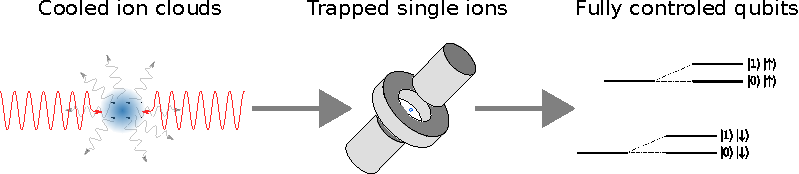
\includegraphics[width=\textwidth]{dw_nutshell.pdf}
\end{frame}

\begin{frame}[t]{David Wineland: Early life}
  \portraitpic{wineland.jpg}
  \visible<3>{
    \textpos{\linewidth}{0cm}{3cm}{\begin{quote}``I knew I was destined to go to
    college and I always kept up my grades to be able to do that''\end{quote}}
  }
  \visible<6>{
    \textpos{\linewidth}{0cm}{3cm}{\begin{quote}``Because I respected my
        classical mechanics teacher so
    much, I asked him about places to apply for graduate school. He recommended
  Harvard, so I applied there.''\end{quote}}
  }
  \begin{minipage}[t][4.5cm][t]{\textwidth-1.5cm}
    \begin{itemize}
      \item<1-> Born near Milwaukee, Wisconsin
      \item<2-> Parents moved to Sacramento, California
      \item<4-> Math Major at University of California, Davis
      \item<5-> Transfer to Berkeley as Physics Major
    \end{itemize}  
  \end{minipage}

  \begin{minipage}[t][0.2\textheight][t]{\textwidth}
    \begin{chronology}[10]{1940}{2016}{\textwidth}{5cm}
      \visible<1>{\event{1944}{24.02.1944}}
      \visible<2>{\event{1947}{'47}}
      \visible<4>{\event{1961}{'61}}
      \visible<5>{\event[1962]{1965}{'62 -- '65}}
    \end{chronology}
  \end{minipage}
\end{frame}

\begin{frame}[t]{David Wineland: Scientific Carreer}
  \portraitpic{wineland.jpg}
  \visible<1>{
    \picpos{6.5cm}{1cm}{1.5cm}{norman_ramsey_group_np.jpg}
  }
  \begin{minipage}[t][4.5cm][t]{\textwidth-1.5cm}
    \begin{itemize}
      \item Master and PhD at Norman Ramseys group in Harvard
      \item<2> Spectroscopy of hyperfine levels of Deuterium
    \end{itemize}  
  \end{minipage}
  \begin{minipage}[t][0.2\textheight][t]{\textwidth}
    \begin{chronology}[10]{1940}{2016}{\textwidth}{5cm}
      \event[1965]{1970}{'65 -- '70}
    \end{chronology}
  \end{minipage}
\end{frame}

\begin{frame}[t]{David Wineland: Scientific Carreer}
  \portraitpic{wineland.jpg}
  \visible<1>{
    \picpos{3cm}{1cm}{1.5cm}{hans_dehmelt_np.jpg}
  }
  \visible<2>{
    \picpos{8cm}{1cm}{2cm}{monoelectron_title.jpg}
  }
  \visible<3>{
    \picpos{8cm}{0.5cm}{2cm}{dw_penning_trap.pdf}
  }
  \visible<4->{
    \picpos{9cm}{1cm}{2.5cm}{dw_monoelectron_plot.pdf}
  }
  \visible<5>{
    \picpos{9cm}{1cm}{2.5cm}{dw_monoelectron_plot1.pdf}
  }
  \visible<6>{
    \picpos{9cm}{1cm}{2.5cm}{dw_monoelectron_plot2.pdf}
  }
  \visible<7>{
    \picpos{9cm}{1cm}{2.5cm}{dw_monoelectron_plot3.pdf}
  }
  \begin{minipage}[t][4.5cm][t]{\textwidth-1.5cm}
    \begin{itemize}
      \item Postdoc in Hans Dehmelts group in Washington
      \item<2-> Trapping single electrons in a Penning trap
    \end{itemize}  
  \end{minipage}
  \begin{minipage}[t][0.2\textheight][t]{\textwidth}
    \visible<1-2>{
      \begin{chronology}[10]{1940}{2016}{\textwidth}{5cm}
        \visible<1>{\event[1970]{1975}{'70 -- '75}}
        \visible<2>{\event{1973}{'73}}
      \end{chronology}
    }
  \end{minipage}
\end{frame}

\begin{frame}[t, noframenumbering]{David Wineland: Scientific Carreer}
  \portraitpic{wineland.jpg}
  \visible<1->{
    \picpos{7cm}{1cm}{2.5cm}{doppler_cooling.pdf}
  }
  \begin{minipage}[t][4.5cm][t]{\textwidth-1.5cm} %TODO Citation of paper
    \begin{itemize}
      \item Postdoc in Hans Dehmelts group in Washington
      \item Idea of laser cooling of ions (Doppler cooling)
    \end{itemize}  
  \end{minipage}
  \begin{minipage}[t][0.2\textheight][t]{\textwidth}
    \begin{chronology}[10]{1940}{2016}{\textwidth}{5cm}
      \visible<>{\event[1970]{1975}{'70 -- '75}}
      \visible<1>{\event{1975}{'75}}
    \end{chronology}
  \end{minipage}
\end{frame}

\begin{frame}[t]{David Wineland: Scientific Carreer}
  \portraitpic{wineland.jpg}
  \visible<2->{
    \picpos{4.5cm}{1cm}{2.1cm}{dw_cs_clock.jpg}
  }
  \begin{minipage}[t][4.5cm][t]{\textwidth-1.5cm} 
    \begin{itemize}
      \item Position at the time and frequency division of the national bureau
        of standards (NBS, later NIST)

      \item In charge of setting up a working Cesium clock
    \end{itemize}  
  \end{minipage}
  \begin{minipage}[t][0.2\textheight][t]{\textwidth}
    \begin{chronology}[10]{1940}{2016}{\textwidth}{5cm}
      \visible<1>{\event[1975]{1977}{'75 -- '77}}
    \end{chronology}
  \end{minipage}
\end{frame}

\begin{frame}[t]{David Wineland: Scientific Carreer}
  \portraitpic{wineland.jpg}
  \visible<1>{
    \picpos{6cm}{1cm}{1.5cm}{dw_group_79.jpg}
  }
  
  \visible<3>{
    \picpos{9cm}{1cm}{2.5cm}{dw_doppler_cooling_title_full.jpg}
  }

  \visible<4-5>{
    \picpos{5.5cm}{0.5cm}{3cm}{dw_laser_cooling_ions_setup.pdf}
  }

  \visible<5>{
    \picpos{5.5cm}{6cm}{3.5cm}{dw_laser_cooling_ions_plot.pdf}
  }

  \visible<6>{
    \picpos{9cm}{1cm}{2.5cm}{dw_doppler_cooling_title.jpg}
  }
  
  \visible<6>{
    \picpos{9cm}{1cm}{4.8cm}{dehmelt_toschek_cooling_title.jpg}
  }
   
  \visible<2>{
    \textpos{\linewidth}{0cm}{3cm}{\begin{quote}``I knew that we had competition
    because I was aware that Dehmelt had taken a sabbatical to work in Peter
Toschek's lab in Heidelberg, with the same goal of demonstrating cooling.''\end{quote}}
  }
  \begin{minipage}[t][4.5cm][t]{\textwidth-1.5cm}
    \begin{itemize}
      \item<1-> Own group at NBS to research trapped ions and lasers
      \item<2-> Taking up the earlier idea of Doppler cooling
    \end{itemize}  
  \end{minipage}
  \begin{minipage}[t][0.2\textheight][t]{\textwidth}
    \visible<1>{
      \begin{chronology}[10]{1940}{2016}{\textwidth}{5cm}
        \event[1977]{2016}{'77 -- '16 }
      \end{chronology}
    }
  \end{minipage}
\end{frame}

\begin{frame}[c]
  \begin{center}
      \Large Trapped single electrons and cooled down ion clouds, what is next?  
  \end{center}
\end{frame}

\begin{frame}[t]{David Wineland: Research}
  \portraitpic{wineland.jpg}
  \visible<1,5>{
    \picpos{9cm}{.7cm}{1.7cm}{dw_single_mg_title.pdf}
  }
  \visible<2-4>{
    \picpos{8cm}{1cm}{1.5cm}{dw_single_mg_plot.pdf}
  }
  \visible<3>{\picpos{8cm}{1cm}{1.5cm}{dw_single_mg_plot1.pdf}}
  \visible<4>{\picpos{8cm}{1cm}{1.5cm}{dw_single_mg_plot2.pdf}}
  \visible<5>{\picpos{9cm}{.7cm}{4.1cm}{dehmelt_mono_ion_title.pdf}}

  \begin{minipage}[t][4.5cm][t]{\textwidth-1.5cm}
    \begin{itemize}
      \item Trapping of single ions
    \end{itemize}  
  \end{minipage}
  \begin{minipage}[t][0.2\textheight][t]{\textwidth}
    \visible<1>{
      \begin{chronology}[10]{1940}{2016}{\textwidth}{5cm}
        \event{1981}{'81 }
        \visible<>{\event{1999}{'99 -- '99}} %this will never be visible, just
      \end{chronology}
    }
  \end{minipage}
\end{frame}

\begin{frame}[t]{David Wineland: Ion Quantum Jumps}
  \portraitpic{wineland.jpg}

  \visible<1>{
    \picpos{8cm}{0.5cm}{1.9cm}{DW_quantum_jumps_title.pdf}
  }

  \visible<2>{\picpos{7.5cm}{0cm}{1.9cm}{dw_quantum_jumps_scheme0.pdf}}
  \visible<3>{\picpos{7.5cm}{0cm}{1.9cm}{dw_quantum_jumps_scheme1.pdf}}
  \visible<4>{\picpos{7.5cm}{0cm}{1.9cm}{dw_quantum_jumps_scheme2.pdf}}
  \visible<4>{\textpos{5cm}{7.5cm}{4.5cm}{\small fluorescence only when ion occupies
    ground state}}
  \visible<5>{\picpos{7.5cm}{0cm}{1.9cm}{dw_quantum_jumps_scheme_level.pdf}}
  
  \visible<5>{
    \picpos{7cm}{2.8cm}{3cm}{DW_quantum_jumps_results.pdf}
    \textpos{6cm}{3cm}{5.5cm}{\small $\rightarrow$ quantum jumps between ground
    and excited state}
  }
  \begin{minipage}[t][4.5cm][t]{\textwidth-1.5cm}
    \begin{itemize}
      \item Quantum jumps of an ions electron shell
    \end{itemize}  
  \end{minipage}
  \begin{minipage}[t][0.2\textheight][t]{\textwidth}
    \visible<1>{
      \begin{chronology}[10]{1940}{2016}{\textwidth}{5cm}
        \event{1986}{'86 }
        \visible<>{\event{1999}{'99 -- '99}} %this will never be visible, just
      \end{chronology}
    }
  \end{minipage}
\end{frame}

\begin{frame}[t]{David Wineland: Research}
  \portraitpic{wineland.jpg}
  \visible<1>{
    \picpos{8cm}{0.5cm}{1.9cm}{dw_recoilless_single_ion_title.pdf}
  }

  %\visible<2>{
  %  \picpos{\textwidth}{0cm}{1.9cm}{dw_quantized_motion_plot.pdf}
  %}
  \begin{minipage}[t][4.5cm][t]{\textwidth-1.5cm}
    \begin{itemize}
      \item Quantized motional states of the ion in the trap can be resolved
        with a tunable laser
    \end{itemize}  
  \end{minipage}
  \begin{minipage}[t][0.2\textheight][t]{\textwidth}
    \visible<1>{
      \begin{chronology}[10]{1940}{2016}{\textwidth}{5cm}
        \event{1987}{'87 }
        \visible<>{\event{1999}{'99 -- '99}} %this will never be visible, just
      \end{chronology}
    }
  \end{minipage}
\end{frame}

\begin{frame}[t]{David Wineland: Research}
  \portraitpic{wineland.jpg}
  \visible<1>{
    \picpos{8cm}{0.5cm}{1.9cm}{DW_zero_point_energy_title.pdf}
  }
  \visible<2>{
    \picpos{\textwidth}{0cm}{1.9cm}{sideband_cooling_scheme_2_0.pdf}
  }
  \visible<3>{
    \picpos{\textwidth}{0cm}{1.9cm}{sideband_cooling_scheme_3.pdf}
  }
  \visible<4>{
    \picpos{\textwidth}{0cm}{1.9cm}{sideband_cooling_scheme_4.pdf}
  }
  \visible<5>{
    \picpos{\textwidth}{0cm}{1.9cm}{sideband_cooling_scheme_5.pdf}
  }
  \visible<6>{
    \picpos{\textwidth}{0cm}{1.9cm}{sideband_cooling_scheme_6.pdf}
  }
  \visible<7>{
    \picpos{\textwidth}{0cm}{1.9cm}{sideband_cooling_scheme_7.pdf}
    \textpos{4cm}{7.5cm}{6cm}{\small $\rightarrow$ Atom cooled to motional ground state}
  }
  \visible<2->{
    \picpos{\textwidth}{0cm}{1.9cm}{sideband_cooling_scheme_states.pdf}
  }
  \begin{minipage}[t][4.5cm][t]{\textwidth-1.5cm}
    \begin{itemize}
      \item Resolved sideband cooling to motional ground state
    \end{itemize}  
  \end{minipage}
  \begin{minipage}[t][0.2\textheight][t]{\textwidth}
    \visible<1>{
      \begin{chronology}[10]{1940}{2016}{\textwidth}{5cm}
      \visible<>{\event{1999}{'99 -- '99}} %this will never be visible, just
        \event{1989}{'89}
      \end{chronology}
    }
  \end{minipage}
\end{frame}


\begin{frame}[t]{David Wineland: Quantum Logic Gate}
  \portraitpic{wineland.jpg}
  \visible<1>{\picpos{9cm}{0.5cm}{1.5cm}{DW_cnot_gate_title.pdf}}
  \visible<2->{\picpos{5cm}{0.8cm}{2.5cm}{qubits.pdf}}
  \visible<2>{\textpos{5cm}{6.4cm}{3.5cm}{internal qubit
    $\begin{cases}\ket{\uparrow} \\ \ket{\downarrow}\end{cases}$}}
  \visible<2>{\textpos{5cm}{7cm}{5cm}{trap qubit
    $\begin{cases}\ket{0} \\ \ket{1}\end{cases}$}}
  \visible<3-5>{\textpos{6cm}{5.4cm}{3.8cm}{\begin{itemize}\item 4 possible pure
      states \item superposition states can be engineered by laser
pulses \item<5> basic logic operations possible\end{itemize}}}
  \visible<4>{\textpos{8cm}{0.8cm}{6cm}{$\ket{0}\ket{\downarrow}
  \xrightarrow[\text{blue sideband}]{\hspace{0.5cm}\pi/2\text{-pulse on}\hspace{0.5cm}}
  \frac{1}{\sqrt{2}}\left( \ket{0}\ket{\downarrow} + \ket{1}\ket{\uparrow}\right)$}}

  \visible<4>{\picpos{5cm}{0.8cm}{2.5cm}{qubits_arrow.pdf}}
  \begin{minipage}[t][4.5cm][t]{\textwidth-1.7cm}
    \begin{itemize}
      \item Use of trapped ion to store and manipulate two qubits
    \end{itemize}  
  \end{minipage}
  \begin{minipage}[t][0.2\textheight][t]{\textwidth}
    \visible<1>{
      \begin{chronology}[10]{1940}{2016}{\textwidth}{5cm}
        \event{1996}{'95 }
        \visible<>{\event{1999}{'99 -- '99}} %this will never be visible, just
      \end{chronology}
    }
  \end{minipage}
\end{frame}

\begin{frame}[t]{David Wineland: Quantum Logic Gate}
  \portraitpic{wineland.jpg}
  \visible<2->{\picpos{4cm}{0.8cm}{2.8cm}{controled_not.pdf}}
  \visible<3->{\picpos{6cm}{5.2cm}{2.8cm}{DW_cnot_gate_truthtable.pdf}}

  \begin{minipage}[t][4.5cm][t]{\textwidth-1.7cm}
    \begin{itemize}
      \item Controled NOT gate (CNOT): flip target qubit ($\ket{\uparrow}$ or
        $\ket{\downarrow}$) only if control qubit ($\ket{0}$ or $\ket{1}$) is $\ket{1}$
    \end{itemize}  
  \end{minipage}
  \begin{minipage}[t][0.2\textheight][t]{\textwidth}
    \visible<>{
      \begin{chronology}[10]{1940}{2016}{\textwidth}{5cm}
        %\event{1996}{'95 }
        \visible<>{\event{1999}{'99 -- '99}} %this will never be visible, just
      \end{chronology}
    }
  \end{minipage}
\end{frame}

  \section{Conclusion}
\label{sec:Conclusion}
Having now visited some of the experiments that Serge Haroche and David Wineland
realized, the similarities between their fields of research have become even more
clear. Theoretically single trapped  ions and atoms in cavities can be 
treated equivalently by applying the Jaynes-Cummings Hamiltonian and the method of Fock states
to describe either the photon number or the quantum number of motion. Also
experimentally we see that to observe the desired quantum mechanical effects both
of them put huge effort into the isolation of single quanta.

To this day Serge Haroche continues to do research in the field of cavity
quantum electrodynamics, some of his current interests being non-local quantum
states and the quantum engineering of Rydberg states, at École Normale
Supérieure in Paris. Also David Wineland continues to be the leader of the ion
storage group at NIST working on high precision time standards and quantum
information processing, this being another interesting parallel between the two.

Especially in association with prestigious prizes, the work of the laureates is
often depicted as the sole performance of extraordinary individuals. At least in
the case of Serge Haroche and David Wineland this is not true, as they both
pointed out in their Nobel lectures~\cite{wineland2012nobel, haroche2012nobel}.
Both of them had important colleagues some of which spent more than forty years
in the laboratories with them and contributed important ideas to their work.
Both of them were lucky to work with great scientists of current and preceding
generations from their very first days of research. Further it is important to
realize what role technological progress played. Without the invention of
tunable lasers, pulsed lasers, ion traps or superconducting materials, none of
the experiments would have been possible. To put it in the words of Serge
Haroche:
\begin{quote}
  ``On the professional side, I have had the luck to embark in a field - atomic
  physics and quantum optics - which has undergone  fantastic  developments
  over this period of time, improving by many orders of magnitudes the
  sensitivity of experiments and the precision of measurements. Thanks to
  advances in laser technology, new domains have been explored, in ultra-low
  temperature physics or in the study of ultrafast phenomena for instance, that
  we could not even imagine at the time I was working for my PhD. I did not work
  myself in many of these fields, but I witnessed these developments as a member
  of a very active and imaginative community of physicists, sharing the
  excitement and the bewilderment brought about by all these spectacular
  advances.''~\cite{shbio}
\end{quote}

This said we end the term paper with the remark that both of the laureates have left an
impressive lifework that was and is definitely worth the study.


  \newpage
  \printbibliography
\end{document}
